\begin{figure}[h]
	\centering
    %     \begin{subfigure}[b]{0.47\textwidth}
    %     	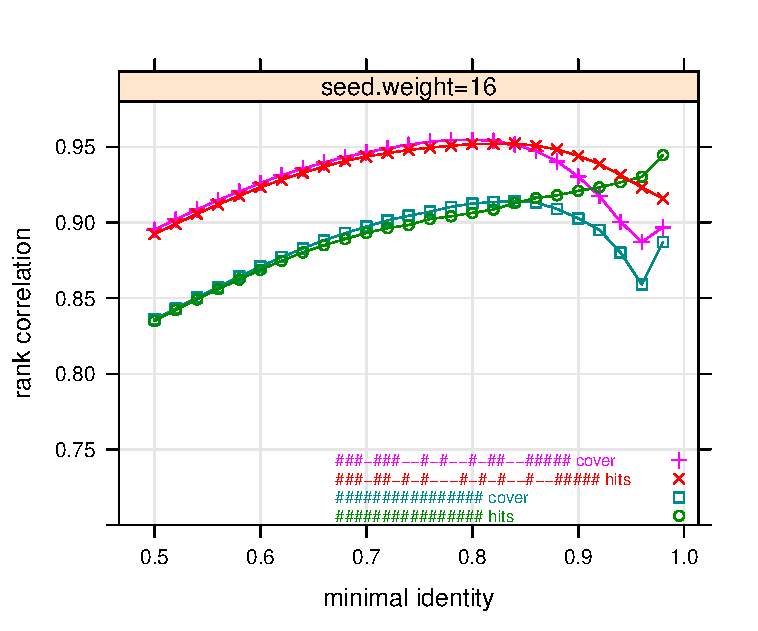
\includegraphics[width=\textwidth]{images/3.2/rank-cor-seed-weight-16.pdf}
    %         \label{weight16}
    % \end{subfigure}
    %     ~    
    % \begin{subfigure}[b]{0.47\textwidth}
    %     	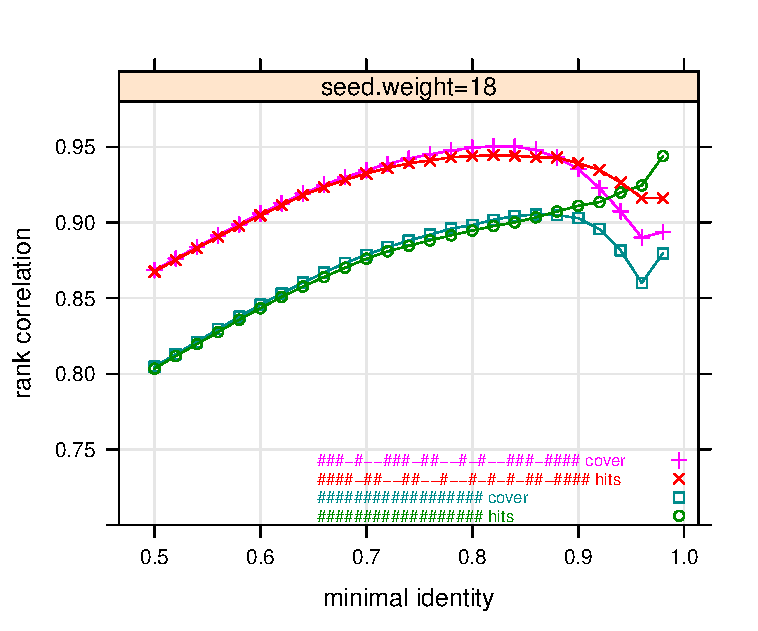
\includegraphics[width=\textwidth]{images/3.2/rank-cor-seed-weight-18.pdf}
    %     \label{weight18}
    %     \end{subfigure}
              
    %     \begin{subfigure}[b]{0.47\textwidth}
    %     	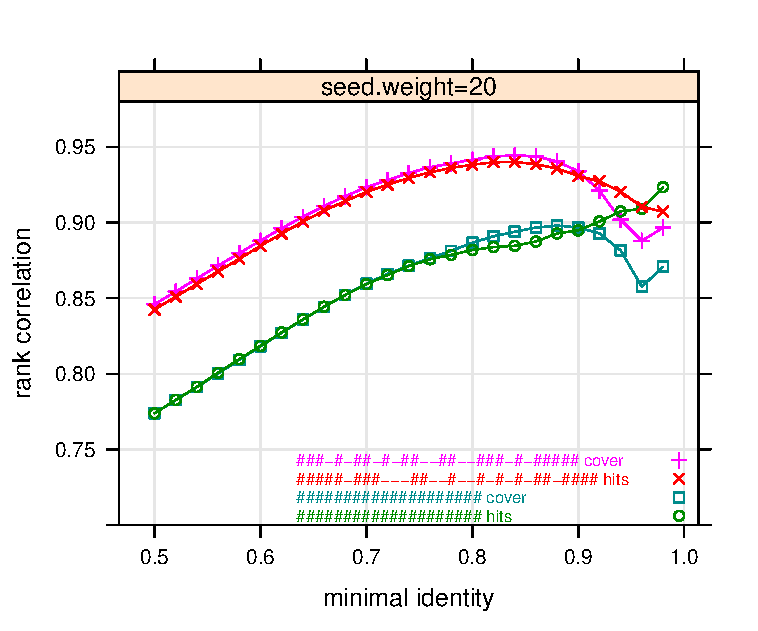
\includegraphics[width=\textwidth]{images/3.2/rank-cor-seed-weight-20.pdf}
    %     \label{weight20}
    %     \end{subfigure}
    %     ~
%	\begin{subfigure}[b]{0.47\textwidth}
		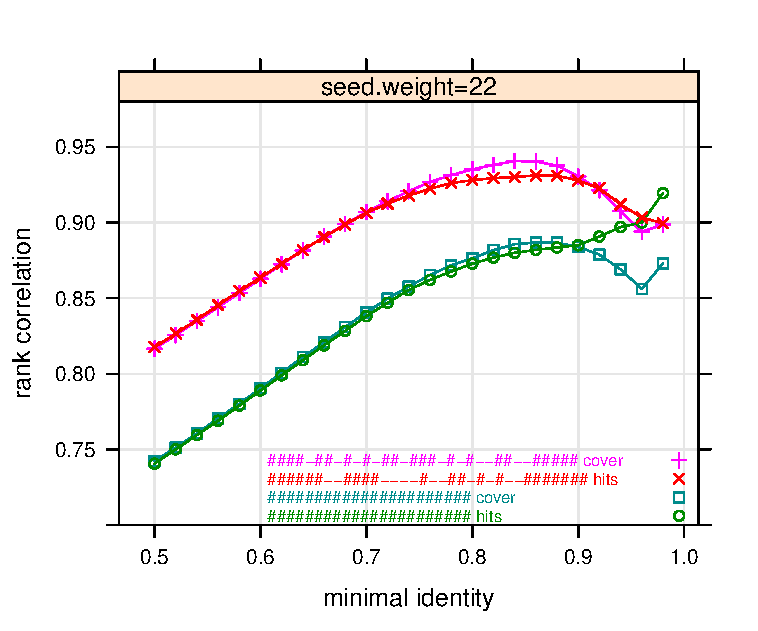
\includegraphics[width=\columnwidth]{images/3.2/rank-cor-seed-weight-22.pdf}
%        \label{weight22}
%	\end{subfigure}\\
              
	% \begin{subfigure}[b]{0.47\textwidth}
	% 	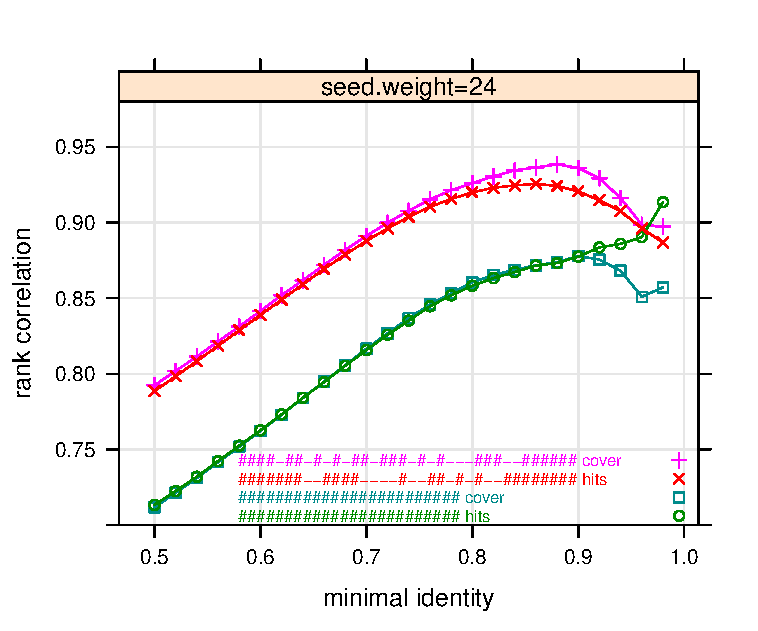
\includegraphics[width=\textwidth]{images/3.2/rank-cor-seed-weight-24.pdf}
        % label{weight24}
	% \end{subfigure}

	\caption{Spearman's rank correlation between score and counts, depending on
  the minimal identity rate. 
% and on whether the seed is contiguous or spaced
}\label{spearman}
\end{figure}
